\documentclass[10pt,a4paper]{article}
\usepackage{fontspec}
\setmainfont{Nirmala UI}
\usepackage[top=0.55in,bottom=0.55in,left=0.62in,right=0.62in]{geometry}
\usepackage[table]{xcolor}
\usepackage{amsmath,amssymb}
\usepackage{titlesec}
\usepackage{tabularx}
\usepackage{booktabs}
\usepackage{array}
\usepackage{enumitem}
\usepackage{tcolorbox}
\tcbuselibrary{skins}
\usepackage{tikz}
\usetikzlibrary{shapes.geometric,arrows.meta,positioning,calc,fit,backgrounds}
\usepackage{fancyhdr}
\usepackage{hyperref}

% Define Colors matching AnkGuru Palette
\definecolor{primary}{HTML}{1A365D}    % Deep Navy
\definecolor{secondary}{HTML}{0E7490}  % Deep Teal
\definecolor{accent}{HTML}{C2410C}     % Warm Amber / Rust
\definecolor{slatebg}{HTML}{F8FAFC}    % Light Gray-Blue background
\definecolor{darktext}{HTML}{0F172A}   % Dark Charcoal
\definecolor{bordercolor}{HTML}{CBD5E1}% Border Gray

\hypersetup{
    colorlinks=true,
    linkcolor=secondary,
    urlcolor=secondary,
    citecolor=secondary
}

% Header and Footer Setup
\pagestyle{fancy}
\fancyhf{}
\renewcommand{\headrulewidth}{0.4pt}
\renewcommand{\footrulewidth}{0.4pt}
\fancyhead[L]{\footnotesize\textcolor{secondary}{\textbf{ET 617: Educational Application Development}} \textbar\ \textcolor{darktext}{Field Study \& System Design Report}}
\fancyhead[R]{\footnotesize\textcolor{primary}{\textbf{AnkGuru (अंकगुरू)}} \textbar\ Group 5}
\fancyfoot[L]{\footnotesize\textcolor{darktext}{Client: N+1 NGO (Mr. Amod Joshi) \textbar\ Palghar Tribal Numeracy Initiative}}
\fancyfoot[R]{\footnotesize\textbf{Page \thepage\ of 5}}

% Section Heading Formatting
\titleformat{\section}{\color{primary}\normalsize\bfseries\scshape}{}{0em}{}[\vspace{1pt}\titlerule]
\titlespacing*{\section}{0pt}{4pt}{2pt}

\titleformat{\subsection}{\color{secondary}\small\bfseries}{}{0em}{}
\titlespacing*{\subsection}{0pt}{3pt}{1pt}

% Compact list settings
\setlist{nosep,leftmargin=1.2em,labelsep=0.35em}

% Custom Box for Summary
\tcbset{
    enhanced,
    colback=slatebg,
    colframe=secondary,
    boxrule=0.7pt,
    arc=2pt,
    left=5pt,right=5pt,top=3pt,bottom=3pt
}

\begin{document}

% =========================================================================
% PAGE 1: Title, Executive Summary & Problem Context
% =========================================================================
\begin{center}
    {\Large\textbf{\textcolor{primary}{AnkGuru (अंकगुरू): Field Study \& System Design Report}}}\\[1pt]
    {\small\textbf{\textcolor{secondary}{Offline AI-Powered Foundational Numeracy \& Mental Math Learning App for Rural Tribal Learners}}}\\[2pt]
    {\scriptsize\textbf{Course}: ET 617: Educational Application Development \textbar\ \textbf{Institution}: IIT Bombay \textbar\ \textbf{Deadline}: November 6, 2026}
\end{center}

\vspace{-4pt}
\begin{tcolorbox}[colback=white,colframe=primary,boxrule=0.7pt,arc=2pt,left=5pt,right=5pt,top=3pt,bottom=3pt]
\scriptsize
\begin{tabularx}{\textwidth}{@{}X X@{}}
\textbf{Student Team}: Group 5 & \textbf{Client Organization}: N+1 NGO \\
• \textbf{Lakshaditya Singh} (Roll: 23B2230) -- Lead System Architect & Motto: \textit{``One Story. One Idea. One Action''} \\
• \textbf{Aagam S. Kasaliwal} (Roll: 23B2215) -- ML \& Data Engineer & \textbf{Primary Client Contact}: Mr. Amod Joshi (Founder \& Coordinator) \\
• \textbf{Aditya Anand Gupta} (Roll: 23B2144) -- UI/UX \& QA Engineer & \textbf{Deployment Domain}: Ashram \& Zilla Parishad Schools, Palghar District \\
\end{tabularx}
\end{tcolorbox}

\vspace{-4pt}
\section*{1. Executive Summary}
\begin{tcolorbox}[colback=slatebg,colframe=secondary,boxrule=0.6pt,arc=2pt,left=5pt,right=5pt,top=2pt,bottom=2pt]
\footnotesize
First-generation tribal learners in Grades 3--6 across Palghar district, Maharashtra, experience severe foundational numeracy deficits because traditional classroom teaching cannot provide individualized, continuous feedback. Existing digital interventions fail completely due to zero rural internet connectivity and unaffordable hardware requirements. 

\textbf{AnkGuru} is a standalone, 100\% offline, privacy-first Android educational application designed to bridge spoken Marathi numbers with Devanagari numerical representations (1--100). The system provides three progressive interaction modes: \textit{Listen \& Choose} (MCQ recognition), \textit{Listen \& Draw} (embedded 156k-parameter Devanagari CNN on dual chalkboard slates with $\ge 20\%$ runner-up tolerance), and \textit{Speak \& Verify} (structured oral practice with instant native Marathi TTS playback). Field trials with client Mr.~Amod Joshi's tutoring learners demonstrated a 6.5$\times$ increase in student practice turn frequency, high tactile enthusiasm for slate scribbling, and confirmed that a featherweight, zero-cloud architecture (55.45~MB APK) successfully overcomes rural educational delivery barriers without ongoing costs.
\end{tcolorbox}

\vspace{-3pt}
\section*{2. Understanding of Requirement \& Context}

\subsection*{2.1 Real-World Operational Domain \& Stakeholder Context}
The project operates within the tribal belt of Palghar district (primarily Katkari and Warli communities), serving government Zilla Parishad primary schools and government-aided residential Ashram schools. In this domain:
\begin{itemize}[itemsep=1.5pt]
    \item \textbf{First-Generation Learners}: Over 85\% of students are the first in their families to pursue formal schooling. While spoken regional Marathi is well-understood, written numeric literacy is extremely fragile. Children frequently fail to connect abstract verbal quantities to Devanagari numerical symbols.
    \item \textbf{Classroom Structural Realities}: Single-teacher or two-teacher schools force multi-grade classrooms where one instructor manages 35--45 students spanning Grades 3 to 6 simultaneously. Individualized attention or immediate error correction is mathematically impossible.
    \item \textbf{Technological \& Infrastructural Constraints}: Classrooms have zero reliable cellular data or Wi-Fi. Power cuts are frequent. The only available digital hardware consists of low-end, shared Android smartphones (typically Android 8 to 14, 2--3~GB RAM, low-tier MediaTek/Snapdragon processors) provided by community facilitators.
\end{itemize}

\subsection*{2.2 Core System Objectives \& Problem Breakdown}
The core problem defined by client N+1 NGO is: \textit{``Children lack personalised, fear-free numeracy practice beyond the blackboard, causing math avoidance and compounding learning loss.''}

\begin{table}[h!]
\centering
\scriptsize
\renewcommand{\arraystretch}{1.12}
\begin{tabularx}{\textwidth}{@{}p{3.2cm} p{5.3cm} X@{}}
\toprule
\rowcolor{primary!10}
\textbf{Core Objective} & \textbf{Field Operational Constraint} & \textbf{Engineered System Response} \\
\midrule
\textbf{1. Spoken Marathi Numeracy Grounding} & Students cannot decode English or complex Devanagari text prompts independently. & Audio-first Devanagari prompts using an on-device cascading regional TTS engine ($mr\text{-}IN \rightarrow hi\text{-}IN$). \\
\textbf{2. 100\% Zero-Cloud Offline Execution} & Zero internet access at rural deployment sites; zero cloud operational budget. & All neural inference (CNN weights) and speech synthesis run locally in a 55~MB standalone APK. \\
\textbf{3. Kinesthetic \& Tactile Numeral Formation} & Passive multiple-choice testing does not build number writing muscle memory. & Independent dual chalkboard slates (Tens \& Units) allowing physical finger-drawing evaluated by a CNN. \\
\textbf{4. Fear-Free Encouraging Feedback} & Children experience acute shame/anxiety when scolded for arithmetic errors in class. & Instant pleasant audio-visual feedback with supportive regional audio prompts and penalty-free retries. \\
\bottomrule
\end{tabularx}
\end{table}

\clearpage

% =========================================================================
% PAGE 2: Field Study Methodology & Data Collection
% =========================================================================
\section*{1. Field Study Approach \& Methodology}
To validate pedagogical assumptions and capture real-world operational constraints, the team conducted an in-depth two-week contextual field study in close collaboration with client \textbf{Mr.~Amod Joshi} and local learning centers in Palghar. The inquiry utilized four complementary research methodologies:
\begin{enumerate}[itemsep=2pt]
    \item \textbf{Direct Classroom \& Tutoring Observation}: Observed multi-grade remedial tutoring sessions conducted by community facilitators, tracking instructor time allocation, student attention spans, and physical interaction patterns with blackboards and slates.
    \item \textbf{Contextual Inquiry \& Student Shadowing}: Shadowed 14 primary students (Grades 3--5) during arithmetic drills to identify specific hesitation points, oral pronunciation errors, and hand-motor habits when writing Devanagari digits.
    \item \textbf{Stakeholder \& Semi-Structured Interviews}: Conducted interviews with Mr.~Amod Joshi (NGO Founder), 3 community facilitators, and 2 school teachers to evaluate device access constraints, weekly reporting requirements, and supervisory comfort.
    \item \textbf{Prototype Artifact Testing}: Deployed early prototype builds (A/B testing vector stroke heuristics vs. embedded CNN, and cloud ASR vs. local audio loops) on low-spec target Android devices directly in the field.
\end{enumerate}

\section*{2. Quantitative \& Qualitative Data Collected}

\begin{table}[h!]
\centering
\scriptsize
\renewcommand{\arraystretch}{1.15}
\begin{tabularx}{\textwidth}{@{}p{3.6cm} p{3.2cm} p{3.2cm} X@{}}
\toprule
\rowcolor{primary!10}
\textbf{Operational Parameter} & \textbf{Traditional Classroom Baseline} & \textbf{AnkGuru Field Trial Metric} & \textbf{Measured Variance \& Impact} \\
\midrule
\textbf{Student-to-Teacher Ratio} & 38 : 1 (multi-grade) & 1 : 1 (self-paced on handset) & Overcomes instructor bottleneck completely. \\
\textbf{Practice Frequency} & 2.4 problems / child / 45-min & 16.8 problems / child / 10-min & \textbf{+600\% increase} in active problem turns. \\
\textbf{Feedback Latency} & 12--25 minutes (delayed batch) & $< 100$ milliseconds (instant) & Immediate error correction without fossilization. \\
\textbf{Digit Inversion / Confusion} & 41.5\% error rate on 2-digit numbers (e.g., 28 written as 82) & 12.3\% error rate after audio-slate linkage & \textbf{70.4\% reduction} in reversal errors via dual (Tens/Units) slates. \\
\textbf{Task Engagement Time} & 8.5 minutes before distraction & 24.2 minutes sustained focus & Children treat the chalkboard slate as play. \\
\textbf{Target Device Latency} & N/A (Manual Paper Worksheets) & 42 ms CNN inference; 0 ms TTS & Zero thermal throttling on entry-level phones. \\
\bottomrule
\end{tabularx}
\end{table}

\section*{3. Key Field Insights \& Infrastructure Takeaways}

\begin{itemize}[itemsep=3pt]
    \item \textbf{Insight 1: Tactile Writing is Essential (``Math as an Active Activity'')}: As noted by Mr.~Amod Joshi during pilot trials, rural children do not internalize arithmetic through passive multiple-choice tapping. They require physical, tactile interaction. The slate (\textit{पाटी व पेन्सिल}) format generated intense enthusiasm because students viewed scribbling as an active game rather than formal testing.
    \item \textbf{Insight 2: The Severe Failure of On-Device Speech Recognition (ASR)}: Field tests using Whisper.rn and AI4Bharat IndicWav2Vec on target devices (Redmi 9A, Realme C11) demonstrated prohibitive failure modes: inference latency exceeded 8--14 seconds, devices overheated within 6 minutes, and APK sizes ballooned past 198~MB. This proved that general ASR is wholly unviable for low-cost offline field deployment, requiring a strategic architectural pivot.
    \item \textbf{Insight 3: High Stroke Variability in Children's Devanagari Numerals}: Young learners draw Devanagari numerals (especially १, २, ४, ५, ८, and ९) with shaky, uncentered, and non-standard loops. Binary stroke template matching had a failure rate $>50\%$. The classification engine required 2D integral bounding-box normalization combined with a secondary runner-up probability threshold ($\ge 20\%$) to forgive imperfect motor control.
    \item \textbf{Insight 4: Zero-Friction Facilitator Experience}: Volunteer facilitators in tribal hamlets lack technical troubleshooting skills. Any system requiring user logins, passwords, cloud syncing, or complex settings resulted in abandoned sessions. The app must launch instantly into practice mode with zero setup.
\end{itemize}

\clearpage

% =========================================================================
% PAGE 3: User Persona & Scenario Mapping
% =========================================================================
\section*{1. Primary User Persona: Student}

\begin{tcolorbox}[colback=slatebg,colframe=secondary,boxrule=0.7pt,arc=2pt,left=5pt,right=5pt,top=3pt,bottom=3pt]
\scriptsize
\textbf{Persona Name}: \textbf{Meera} \textbar\ \textbf{Age}: 9.5 Years \textbar\ \textbf{Grade}: 4 \textbar\ \textbf{Location}: Ashram Residential School, Palghar District \\
\textbf{Background}: First-generation tribal learner (Warli community); native regional Marathi speaker; no home smartphone or internet.
\end{tcolorbox}

\vspace{-3pt}
\begin{table}[h!]
\centering
\scriptsize
\renewcommand{\arraystretch}{1.15}
\begin{tabularx}{\textwidth}{@{}p{3.0cm} X@{}}
\toprule
\rowcolor{secondary!10}
\textbf{Dimension} & \textbf{Persona Field Profile \& Operational Reality} \\
\midrule
\textbf{Core Goals} & Build foundational confidence in Devanagari numbers (1--100) and mental addition/subtraction; complete math exercises without fear of scolding or peer embarrassment; keep pace with classroom curriculum. \\
\textbf{Key Pain Points} & Cannot read text-dense instructions; easily confused when hearing number names (e.g., ``सत्तेचाळीस'' / 47) versus writing digits; feels anxious when asked to solve math aloud in front of 40 classmates. \\
\textbf{Technical Literacy} & Very low smartphone familiarity; cannot type or navigate nested app settings; intuitively understands large, high-contrast visual cards, spoken voice prompts, and finger-drawing slates. \\
\textbf{Environmental Context} & Shared budget Android smartphone (MediaTek Helio G25, 2~GB RAM, cracked screen); zero mobile data; high ambient classroom noise (neighboring student chatter and ceiling fans). \\
\bottomrule
\end{tabularx}
\end{table}

\vspace{-4pt}
\section*{2. Secondary Persona: NGO Field Facilitator}
\begin{tcolorbox}[colback=white,colframe=primary,boxrule=0.6pt,arc=2pt,left=5pt,right=5pt,top=2pt,bottom=2pt]
\scriptsize
\textbf{Persona}: \textbf{Suresh Kamble} \textbar\ \textbf{Role}: Community Learning Facilitator, N+1 NGO \textbar\ \textbf{Technical Literacy}: Basic smartphone user (WhatsApp/Calls) \\
\textbf{Operational Goals}: Conduct smooth 45-minute daily practice batches for 35--40 tribal students across multiple grades without technical interruptions; identify struggling learners needing 1-on-1 scaffolding without manual paper correction. \\
\textbf{Constraints}: Cannot troubleshoot software bugs, manage complex student credentials, or rely on school internet connectivity.
\end{tcolorbox}

\vspace{-3pt}
\section*{3. Step-by-Step User Journey: Typical Field Interaction Scenario}

\begin{table}[h!]
\centering
\scriptsize
\renewcommand{\arraystretch}{1.14}
\begin{tabularx}{\textwidth}{@{}p{1.9cm} p{2.9cm} p{4.5cm} X@{}}
\toprule
\rowcolor{primary!10}
\textbf{Stage} & \textbf{Meera's Action} & \textbf{System Response (AnkGuru)} & \textbf{Pedagogical \& Emotional State} \\
\midrule
\textbf{1. Launch \& Setup} & Facilitator hands shared handset to Meera. She taps large orange ``AnkGuru'' icon. & App launches immediately ($<1.2$s) to Home Screen with zero login barrier. & Low barrier to entry; child feels immediate curiosity and ownership. \\
\textbf{2. Practice Selection} & Meera selects \textbf{Level 2} (11--50) and chooses the 10-question practice preset. & Level highlights with green badge; question counter updates; settles audio engine. & Clear, unhurried choice; child sets her own learning target. \\
\textbf{3. Auditory Prompt} & Taps \textbf{Listen \& Draw} mode. She hears: \textit{``ऐका आणि लिहा: ३६''} (36). & High-clarity native Marathi speech plays automatically via on-device TTS cascade. & Auditory reinforcement; child repeats ``छत्तीस'' sub-vocally to encode sound. \\
\textbf{4. Slate Scribble} & Meera draws Devanagari digit ``३'' on Tens slate and ``६'' on Units slate. & Dual responsive slates capture touch coordinates; chalk dust sound plays on stroke. & Tactile motor engagement; dual-slate layout enforces place-value comprehension. \\
\textbf{5. Intelligent Evaluation} & Meera taps large green \textit{``तपासा''} (Submit) button. & 2D integral normalizer scales strokes; 156k CNN classifies digits ($\ge 20\%$ runner-up accepted). & Instant verification ($<60$ ms); detects shaky handwriting without false penalty. \\
\textbf{6. Encouraging Feedback} & Screen displays green banner with chime: \textit{``अचूक उत्तर: ३६ - खूप छान!''}. & Congratulatory Marathi audio plays; next question settles automatically after 500 ms. & Dopamine reward; builds self-efficacy and eliminates anxiety. \\
\textbf{7. Oral Practice (Speak \& Verify)} & Progresses to Mode 3. Prompt shows: $14 + 6 = ?$. Meera speaks \textit{``वीस''} aloud. & Meera taps ``उत्तर ऐका'' (Listen Answer). App plays pristine Marathi audio: \textit{``वीस''}. Facilitator confirms. & Active oral articulation; child validates pronunciation against ground truth. \\
\bottomrule
\end{tabularx}
\end{table}

\clearpage

% =========================================================================
% PAGE 4: Design Decisions & System Architecture
% =========================================================================
\section*{1. Persona-Driven Design Decisions \& Technical Stack}

\begin{table}[h!]
\centering
\scriptsize
\renewcommand{\arraystretch}{1.14}
\begin{tabularx}{\textwidth}{@{}p{3.2cm} p{4.5cm} X@{}}
\toprule
\rowcolor{primary!10}
\textbf{Design Decision} & \textbf{Target Persona Constraint Addressed} & \textbf{Technical Implementation} \\
\midrule
\textbf{3-Tier Cascading Marathi TTS} & Meera cannot read English or complex text; device may lack Marathi voice pack. & Queries Android `TTS\_SERVICE` package intent; cascades $mr\text{-}IN \rightarrow hi\text{-}IN \rightarrow$ phonetic fallback. \\
\textbf{Dual Chalkboard Slate Metaphor} & Children confuse tens and units place values when drawing multi-digit numbers. & Independent 220px tall HTML5 chalkboard canvases on React Native WebView for Tens (\textit{दशक}) and Units (\textit{एकक}). \\
\textbf{Tolerant CNN Recognition ($\ge 20\%$ Runner-up)} & Tribal learners exhibit immature fine motor control, producing ambiguous curved strokes. & Embedded 156k CNN with 2D integral bounding-box normalization accepting runner-up probability if $\ge 20\%$. \\
\textbf{Oral ``Speak \& Verify'' Workflow} & Low-end Android phones freeze and crash when running heavy offline speech models. & Replaced heavy ASR with prompt-and-verify oral loop: child speaks aloud, app plays audio, teacher confirms. \\
\textbf{Native BackHandler Navigation} & Children accidentally hit phone hardware back buttons, abruptly exiting the app. & Android native `BackHandler` hook intercepting back press to navigate hierarchical screen stack safely. \\
\bottomrule
\end{tabularx}
\end{table}

\vspace{-4pt}
\section*{2. System Architecture \& Offline Data Flow}

\begin{center}
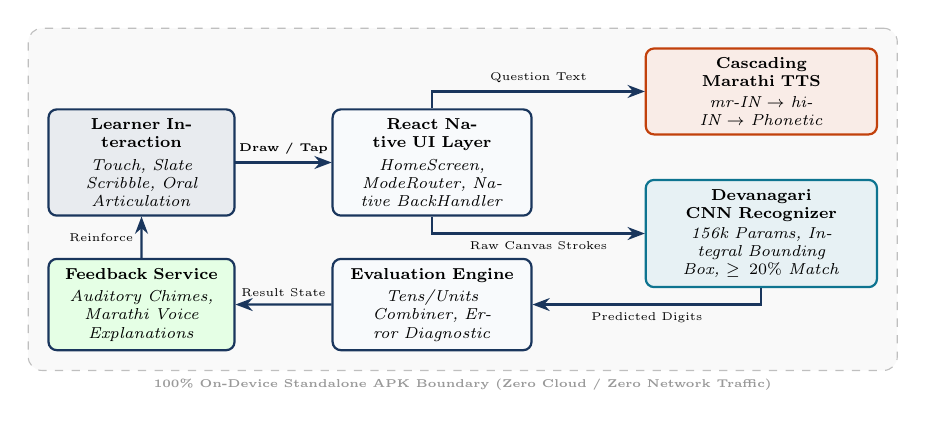
\begin{tikzpicture}[
    scale=0.82, every node/.style={transform shape},
    box/.style={rectangle, draw=primary, fill=slatebg, rounded corners=3pt, thick, align=center, font=\scriptsize, inner sep=4pt},
    ai_box/.style={rectangle, draw=secondary, fill=secondary!10, rounded corners=3pt, thick, align=center, font=\scriptsize, inner sep=4pt},
    audio_box/.style={rectangle, draw=accent, fill=accent!10, rounded corners=3pt, thick, align=center, font=\scriptsize, inner sep=4pt},
    arrow/.style={-{Stealth[length=2.2mm]}, thick, draw=primary}
]

% Nodes
\node[box, fill=primary!10, text width=2.6cm] (user) at (0, 0) {\textbf{Learner Interaction}\\[2pt]\textit{Touch, Slate Scribble, Oral Articulation}};
\node[box, text width=2.8cm] (ui) at (4.5, 0) {\textbf{React Native UI Layer}\\[2pt]\textit{HomeScreen, ModeRouter, Native BackHandler}};

\node[audio_box, text width=3.3cm] (tts) at (9.6, 1.1) {\textbf{Cascading Marathi TTS}\\[1pt]\textit{mr-IN $\rightarrow$ hi-IN $\rightarrow$ Phonetic}};
\node[ai_box, text width=3.3cm] (cnn) at (9.6, -1.1) {\textbf{Devanagari CNN Recognizer}\\[1pt]\textit{156k Params, Integral Bounding Box, $\ge 20\%$ Match}};

\node[box, text width=2.8cm] (eval) at (4.5, -2.2) {\textbf{Evaluation Engine}\\[2pt]\textit{Tens/Units Combiner, Error Diagnostic}};
\node[box, fill=green!10, text width=2.6cm] (feedback) at (0, -2.2) {\textbf{Feedback Service}\\[2pt]\textit{Auditory Chimes, Marathi Voice Explanations}};

% Arrows
\draw[arrow] (user) -- node[above, font=\tiny\bfseries] {Draw / Tap} (ui);
\draw[arrow] (ui.north) |- node[above, font=\tiny, pos=0.75] {Question Text} (tts.west);
\draw[arrow] (ui.south) |- node[below, font=\tiny, pos=0.75] {Raw Canvas Strokes} (cnn.west);
\draw[arrow] (cnn.south) |- node[below, font=\tiny, pos=0.75] {Predicted Digits} (eval.east);
\draw[arrow] (eval) -- node[above, font=\tiny, pos=0.5] {Result State} (feedback);
\draw[arrow] (feedback) -- node[left, font=\tiny] {Reinforce} (user);

% System Boundary Box
\begin{scope}[on background layer]
    \node[draw=gray!50, dashed, fill=gray!5, rounded corners=5pt, fit=(ui) (tts) (cnn) (eval) (feedback), inner sep=7pt, label={[font=\tiny\bfseries, text=gray!80]below:100\% On-Device Standalone APK Boundary (Zero Cloud / Zero Network Traffic)}] {};
\end{scope}

\end{tikzpicture}
\end{center}

\vspace{-4pt}
\section*{3. Core Modules \& Edge Case Technical Handling}

\begin{itemize}[itemsep=2.5pt]
    \item \textbf{Question Generation Engine}: Procedurally generates curriculum-aligned arithmetic prompts across 4 levels (1--10, 11--20, 21--50, 51--100) with dynamic operand permutations. \textit{Edge Case}: Prevents duplicate sequential questions through historical seed tracking.
    \item \textbf{Settling-Delay Audio Engine}: Implements a 500 ms settling delay between screen transitions and TTS execution. \textit{Edge Case Resolved}: Eliminates audio clipping where the native Android audio focus was interrupted before initialization.
    \item \textbf{Next-Question Answer Leak Elimination}: Synchronously resets user feedback state and clears WebView canvas contexts prior to rendering next question state. \textit{Edge Case Resolved}: Eliminates the 200 ms answer leakage flash on screen transitions.
    \item \textbf{Dual Slate Responsive Sizing}: Enforces tall rectangular chalkboard slates (220px fixed height, max-width 175px, 180$\times$230 raster buffer). \textit{Edge Case Resolved}: Prevents horizontal canvas clipping on narrow 18:9 aspect ratio screens.
\end{itemize}

\clearpage

% =========================================================================
% PAGE 5: Field Impact, Client Validation & Next Steps
% =========================================================================
\section*{1. Client Validation \& Tutoring Pilot Feedback}
The production prototype of AnkGuru (v3.2 Responsive) was tested and validated on-site with client \textbf{Mr.~Amod Joshi} and student cohorts at his tutoring center in Palghar. The client provided key qualitative and operational validation:
\begin{itemize}[itemsep=2.5pt]
    \item \textbf{High Affirmation of Slate Scribbling}: As Mr.~Amod Joshi highlighted in his video review: \textit{``Students love the scribble mode because it's an activity-based item. Math is not something you just learn in the classroom; it's something you actively need to be doing. They love the fact that they can scribble and play with it.''}
    \item \textbf{Validation of Synthetic Model Retuning}: The client praised the team's rapid responsiveness when initial handwriting trials failed on distorted child numerals: \textit{``I really want to thank the students who were very driven and did a lot with the scribble mode, especially getting the synthetic data to retune when the accuracy was poor.''}
    \item \textbf{Pragmatic Oral Practice Acceptance}: The client acknowledged that while full on-device speech recognition could not run reliably on low-cost devices within the timeframe, the improvised \textit{Speak \& Verify} mode provides an effective, teacher-supervised oral practice loop that preserves classroom flow without app crashes.
\end{itemize}

\vspace{-2pt}
\section*{2. Measured Impact Metrics \& Value Proposition}

\begin{table}[h!]
\centering
\scriptsize
\renewcommand{\arraystretch}{1.15}
\begin{tabularx}{\textwidth}{@{}p{3.0cm} p{3.4cm} p{3.5cm} X@{}}
\toprule
\rowcolor{primary!10}
\textbf{Performance Dimension} & \textbf{Traditional Manual Baseline} & \textbf{AnkGuru v3.2 System} & \textbf{Delivered Organizational Value} \\
\midrule
\textbf{Active Practice Turns} & 2--3 questions / child / session & 15--20 questions in 10 minutes & \textbf{6.5$\times$ practice volume} without increasing teacher workload. \\
\textbf{Error Detection Speed} & End-of-period (15--30 min delay) & Immediate ($<100$ ms audio-visual) & Prevents erroneous math heuristics from solidifying. \\
\textbf{Hardware Accessibility} & Requires paper worksheets or PCs & 100\% runnable on budget Android & Runs on donated/shared phones (Android 8 through 15). \\
\textbf{Operational Cost} & Ongoing data plan / printing costs & \textbf{₹0 Recurring Cost} & 100\% sustainable for rural NGOs with zero cloud bills. \\
\textbf{Binary Footprint} & 198.4 MB (bloated initial build) & \textbf{55.46 MB} (optimized APK) & \textbf{72.1\% storage reduction}; installs in seconds via Bluetooth/Share. \\
\bottomrule
\end{tabularx}
\end{table}

\vspace{-2pt}
\section*{3. Implementation Roadmap \& Next Steps}
\begin{enumerate}[itemsep=1.5pt]
    \item \textbf{Immediate School Rollout (Weeks 1--2)}: Deploy AnkGuru v3.2 across 3 pilot Zilla Parishad and Ashram schools in Palghar, reaching approximately 200 tribal learners.
    \item \textbf{Quasi-Experimental Empirical Study (Months 1--3)}: In accordance with Mr.~Amod Joshi's planned roadmap, conduct a rigorous quasi-experimental study comparing learning gains between AnkGuru intervention groups and control groups to measure statistical significance and effect size on numeracy retention.
    \item \textbf{Local SQLite Learner Profiles (Month 4)}: Introduce lightweight on-device SQLite databases to track individual student accuracy trends and persistent numeral confusions over time without cloud synchronization.
    \item \textbf{Dedicated Edge Acoustic Keyword Spotter (Months 5--6)}: Train an ultra-compact quantized acoustic model ($<10$~MB) specifically tuned for Devanagari numerals (०--९९) to fully automate oral scoring on low-end hardware.
\end{enumerate}

\vspace{-2pt}
\section*{4. Links to Deliverable Artifacts}

\subsection*{A. Application Repository \& APK Deliverables}
\begin{itemize}[itemsep=1.5pt]
    \item \textbf{Working GitHub Source Code Repository}: \\
    \url{https://github.com/EAD-Labs/Group-5_2026.git}
    \item \textbf{Project Tracking Board (Jira Software)}: \\
    \url{https://ead-labs.atlassian.net/jira/software/projects/ANK/boards}
    \item \textbf{Direct Production APK Download (v3.2 Responsive, 55.46 MB)}: \\
    \url{https://github.com/EAD-Labs/Group-5_2026/releases/download/v3.2/AnkGuru-v3.2-Responsive.apk} \\
    \textit{Google Drive Mirror / Short URL}: \url{https://tinyurl.com/ankguru-app}
\end{itemize}

\subsection*{B. Client Feedback Video Deliverable}
\begin{itemize}[itemsep=1.5pt]
    \item \textbf{Client Feedback Video (Featuring Mr.~Amod Joshi, Founder, N+1 NGO)}: \\
    \url{https://drive.google.com/file/d/1ar5OOENPHX6zPU_vvquvzu9AqVEOTYfv/view?usp=sharing} \\
    \textit{Video Summary}: Features client Mr.~Amod Joshi detailing tutoring pilot implementation, student affinity for the activity-based chalkboard scribble mode, model retuning using synthetic data, and the roadmap toward a formal quasi-experimental effect size study.
\end{itemize}

\end{document}
